\chapter{Opis Implementacji}
\label{chapter:4}

\section{Architektura rozwiązania}

\emph{Poker Master Tool} składa się z trzech odrębnych modułów:
\begin{itemize}
    \item Backend --- część serwerowa odpowiedzialna obsługę żądań HTTP
    \item Silnik gry --- moduł służący do obliczeń układów z wykorzystaniem ewaluatora \emph{TwoPlusTwo}
    \item Frontend --- widok użytkownika aplikacji webowej
\end{itemize}

Kod źródłowy aplikacji dostępny jest jako repozytorium git pod adresem \\ \href{https://github.com/bartoszputek/poker-master-tool/}{https://github.com/bartoszputek/poker-master-tool/}.

Do szybkiego uruchomienia aplikacji na lokalnej maszynie należy zainstalować oprogramowanie Docker, służące do wirtualizacji kontenerów. Aby uruchomić aplikację należy zainstalować sklonować repozytorium oraz wykonać polecenie ---
\verb+docker-compose up+.

Innym sposobem na zbudowanie projektu jest zainstalowanie środowiska uruchomieniowego Node.js i wykonanie kolejnych poleceń:

\begin{Verbatim}[numbers=left,xleftmargin=5mm, frame=single]
npm install 
npm run build:all
npm run start
\end{Verbatim}

Po uruchomieniu aplikacja będzie dostępna jako serwer HTTP pod adresem lokalanym \verb+http://localhost:3000+.

Repozytorium zawiera testy jednostkowe oraz integracyjne umieszczone w katalogu \verb+tests+. Testami jednostkowymi zostały pokryte wszystkie klasy poza klasami fasadowymi, które obudowują funkcje standardowe oraz biblioteki zewnętrzne w wygodny interfejs. Testy zostały napisane według zasad szkoły Londyńskiej \cite{mocks-arent-stubs} z użyciem narzędzi do imitowania (ang. mock/stub) zależności, testując zachowanie i interakcje pomiędzy obiektami. Uruchomienie testów wymaga wykonania polecenia \verb+npm run test+.

\begin{table}[htbp]
    \centering
    \begin{tabular}{lll}
        Język & Pliki & Liczba linii \\
        \midrule
        TypeScript      &    36  & 1621  \\
        JavaScript      &    18  & 745   \\
        C++             &    5   & 597  \\
        C/C++ Header    &    4   & 439 \\
        HTML            &    1  & 414 \\
        CSS             &    5  & 317  \\
        JSON            &    4  & 143  \\
        YAML            &    2  & 57 \\
        Dockerfile      &    1  & 14 \\
        make            &    1  & 6 \\
        \bottomrule
        Razem           &    77 & 4353 \\
        \bottomrule
    \end{tabular}
    \caption{\label{tab:code-statistics}Statystyki kodu wygenerowane za pomocą narzędzia cloc}
\end{table}

\section{Aplikacja serwerowa}

Aplikacja serwerowa została napisana w statycznie typowanym języku TypeScript kompilowanym do języka JavaScript z użyciem biblioteki Express.js. Serwer działa w środowisku uruchomieniowym Node.js. Kod źródłowy modułu backendowego został umieszczony w katalogu \verb+src+.

Aplikacja serwerowa ma za zadanie:
\begin{itemize}
    \item Przyjmować żądania HTTP
    \item Serwować widok klienta w formie statycznie skompilowanych plików
    \item Logować działanie aplikacji 
    \item Przechowywać w pamięci Cache ostatnie zapytania w celu optymalizacji
    \item Obsługiwać błędy aplikacyjne oraz programistyczne
\end{itemize}

Aplikacja wystawia jeden REST'owy endpoint POST pod adresem / , którego celem jest zwrócenie informacji o szansie wygranych, porażek oraz szansie uzyskania poszczególnych układów przez graczy. Endpoint oczekuje dostarczenia danych o kartach graczy, wspólnych oraz kart martwych, które nie biorą udziału w obliczeniach.

\begin{figure}[hb]
    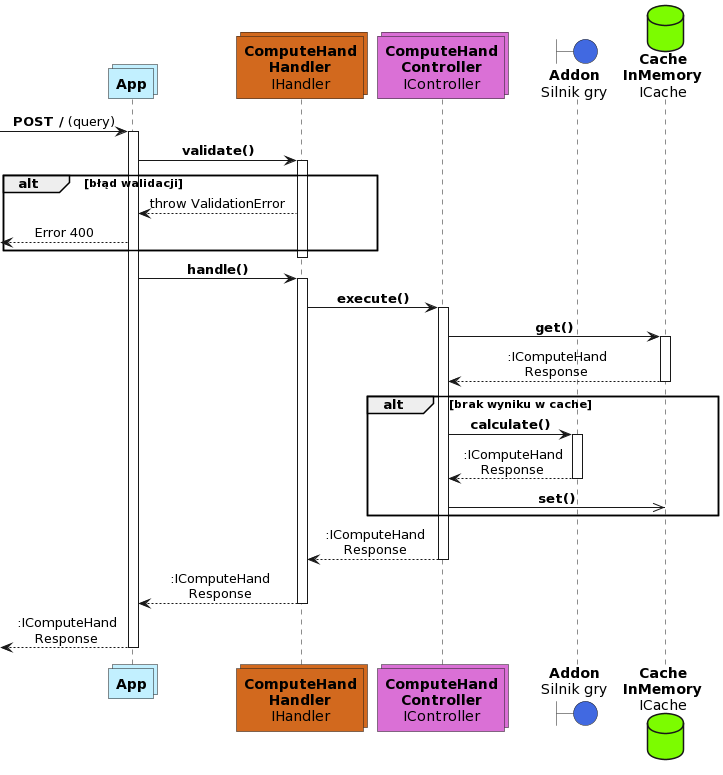
\includegraphics[width=\textwidth]{plantuml/out/backend-sequence-diagram.png}
    \caption{Diagram sekwencji prezentujący interakcję pomiędzy obiektami podczas wywołania metody POST na ścieżkę /. }
    \label{fig:backend-sequence-diagram}
\end{figure}

Po otrzymaniu żądania następuje walidacja danych. Jeżeli takie samo żądanie zostało wykonane niedawno, wynik zostanie zwrócony z pamięci podręcznej (cache) w celu przyspieszenia działania programu. W przeciwnym wypadku obliczany jest wynik za pomocą silnika gry.

\section{Silnik gry}

Silnik gry, wykorzystywany do kalkulacji układów to natywny moduł C++ napisany jako rozszerzenie Node.js. Algorytm wykorzystany do generacji grafu został napisany przez autorów ewaluatora \emph{TwoPlusTwo}, z naniesionymi modyfikacjami poprawiającymi czytelność oraz szybkość działania z wykorzystaniem standardu C++ 17.
Decyzja o wykorzystaniu rozszerzenia została podjęta z przyczyn wydajnościowych, odpowiednik algorytmu w języku JavaScript był zbyt wolny dla pesymistycznych przypadków. 

Przed rozpoczęciem kalkulacji, poleceniem \verb+npm run addon:generate-table+. należy zbudować graf. Następnie, graf musi zostać wczytany do pamięci aplikacji korzystając z funkcji rozszerzenia \verb+initLookUpTable()+ .

Dla silnika gry zostały napisane testy wydajnościowe, które zwracają czasy obliczeń dla wcześniej przygotowanych przypadków użycia. Uruchomienie testów wymaga skorzystania z polecenia \verb+npm run test:performance+.

Rozszerzenie zostało obudowane fasadą upraszczającą korzystanie z obliczeń silnika oraz walidującą poprawność danych wejściowych. Rozszerzenia wymagają mapowania typów --- do tego zadania zostało stworzone proxy. 

\begin{figure}[hb]
    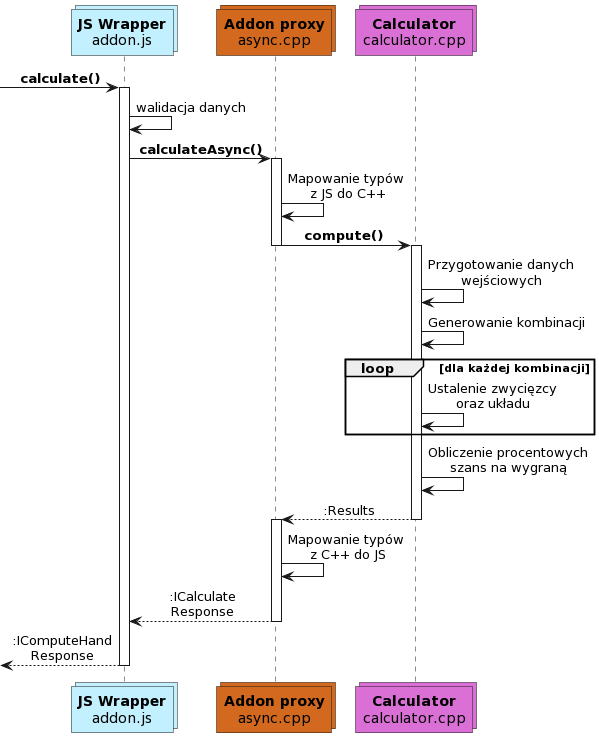
\includegraphics[width=\textwidth]{plantuml/out/engine-sequence-diagram.png}
    \caption{Diagram sekwencji prezentujący przepływ informacji podczas wywołania funkcji calculate(). }
    \label{fig:engine-sequence-diagram}
\end{figure}

\clearpage

\section{Aplikacja klienta}

Rolą aplikacji klienta jest udostępnienie interfejsu przyjaznego dla użytkownika. Widok dostosowuje się do szerokości ekranów urządzeń mobilnych oraz umożliwia obsługę kalkulatora za pomocą klawiatury. Część frontendowa zaprojektowana jest z użyciem technologii JavaScript/HTML/CSS oraz Webpack, który jest narzędziem do budowania projektu (ang. bundler). Kod źródłowy modułu znajduje się w katalogu \verb+frontend+.

Kod podzielony jest na niezależne komponenty, zgodnie z zasadą pojedynczej odpowiedzialności. Widoki utrzymywane są jako klasy \verb+View+, komponenty logiczne umieszczone są w klasach \verb+Controller+, a tymczasowy stan aplikacji utrzymywany jest w repozytoriach. 

Na podstawie stanu aplikacji podejmowana jest decyzja o wykonania żądania \verb+POST /+ i wyświetleniu odpowiedzi. Żądanie wykonywane jest gdy:
\begin{enumerate}
    \item Każdy z graczy jest gotowy (liczba jego kart to 0 lub 2)
    \item Gotowy jest co najmniej jeden gracz
    \item Liczba kart wspólnych jest zgodna z poszczególnymi licytacjami (0/3/4/5)
\end{enumerate}

Wykorzystując powyższą logikę unikamy wykonywania błędnych żądań oraz nie używamy nadmiernie zasobów obliczeniowych serwera.

\begin{figure}[hb]
    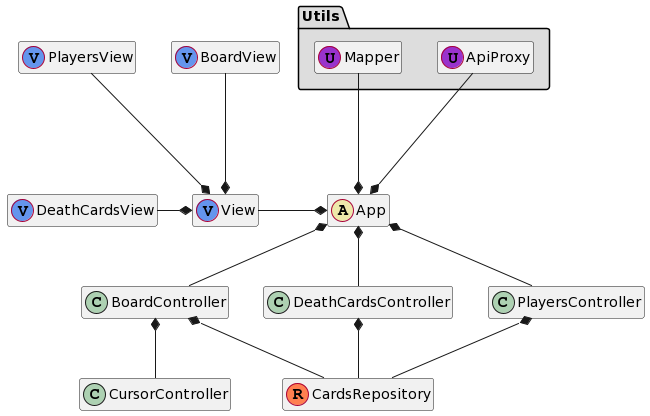
\includegraphics[width=\textwidth]{plantuml/out/frontened-class-diagram.png}
    \caption{Diagram klas wykorzystywanych przez aplikację klienta. }
    \label{fig:frontened-class-diagram}
\end{figure}